\chapter{Интерактивный агент}

Как упоминалось ранее, академические планирующие агенты нацелены на полностью автономную работу. Основной критерий производительности для них - скорость построения оптимального плана.

В случае, когда агент, кроме выполнения последовательности действий,
должен взаимодействовать с другими агентами, в качестве которых могут
выступать пользователи, возникают две новых задачи:

\begin{itemize*}
\item
  Диалог. Мультиагентная среда предполагает взаимодействие с другими
  участниками для получения наилучших результатов.
\item
  Онлайн-планирование. Свойство динамичности проблемной среды требует
  регулярного перестроения плана в условиях изменения начальных и
  конечных условий поставленной задачи.
\end{itemize*}

\subsubsection{Вопросы}

Введем новый вид действий под названием \emph{вопрос}. Изменениям всегда
будет подвергаться только один признак. В качестве предусловия будем
полагать, что значения выбранного признака неизвестно. Вопрос порождает
две дуги из текущего доверительного состояния, соответствующие возможным
полученным значениям признака. Фактически, мы инкапсулируем два
различных действия в одном. Например, для вопроса о значении признака
$L$:

\begin{verbatim}
(: action L_yes :precondition (L?) :effect (L) )

(: action L_no :precondition (L?) :effect (~L) )
\end{verbatim}

Для избежания избыточности в PDDL-описании проблемной среды вопросы явно
указываться не будут.

\subsubsection{Интерактивное планирование}

В мультиагентной проблемной среде агент фактически разбивается на
несколько. Некоторые из них взаимодействуют с другими агентами в среде.
Мы можем выделить:

\begin{itemize*}
\item
  Планирующий агент. Действует в статической одноагентной среде,
  заданной в виде PDDL описания предметной области и поставленной задачи
  планирования. Цель агента - построение условного плана
\item
  Диалоговый агент. Обладает исполнительными механизмами ведения диалога
  с другими агентами. Действует в динамической мультиагентной среде в
  соответствии с программой заданной условным планом. При изменении
  задачи обращается к планирующему агенту.
\end{itemize*}

\section{Планирующий агент. Построение условного плана}

\begin{figure}[h]
 \centering
 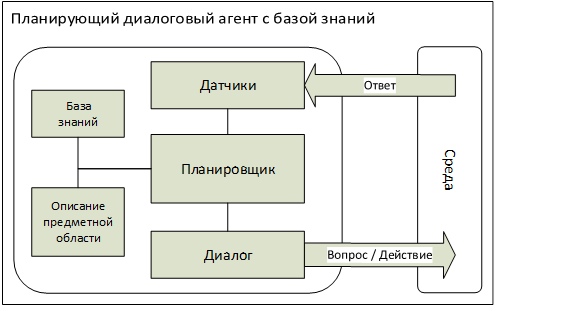
\includegraphics{dialogagent.png}
 \caption{Схема планирующего диалогового агента с базой знаний}
\end{figure}

Условный план строится рекурсивно из начального состояния. Приведем неформальное описание алгоритма:

\begin{enumerate}
\item
  Определить начальное доверительное состояние
\item
  Построить преемников начального состояния

  \begin{enumerate*}
  \item
    Ветвления по неизвестным признакам
  \item
    Гарантированный путь до цели
  \item
    Смешанный путь до цели
  \end{enumerate*}
\item
  Добавить все полученные вершины в очередь
\item
  Если очередь не пуста, выбрать ее вершину в качестве начального
  состояния и перейти на шаг 2
\item
  Если очередь пуста - план построен.
\end{enumerate}

\subsection{Поиск начального состояния}

Как описано далее, в каждом новом состоянии необходимо множество раз решать задачу SAT с участием конъюнкции участвующих в описании состояния среды. Как правило, не все они изменяются в процессе выполнения условного плана. Поэтому для ускорения дальнейшей работы алгоритма целесообразно попытаться исключить те из предикатов, значения которых не принимаются во внимание.

Для этого предлагается подход с поиском пути из целевого состояния в какое-либо подмножество начального, состоящего целиком из действий. На каждом шаге алгоритма предикаты, отсутствующие в описании целевого или начального состояний, добавляются в специальное множество. Далее начальное состояние, заданное в описании задачи планирования, дополняется этим множеством с пометкой, что каждый предикат имеет неизвестное значение.

В дальнейшем, если при прямом поиске из начального состояния алгоритм сталкивается с ситуацией, когда изменяется значение предиката, не участвующего в выборке, начального состояния дополняется и производится поиск неучтенных веток условного плана, возможно ведущих к цели.

Открытым остается вопрос выбора равнозначных наборов предикатов, соответствующих различным независимым путям из начального в целевое состояние.


\begin{algorithm}
 \caption{Обратный поиск начального состояния из целевого}
 \begin{algorithmic}
  \Require predicates, actions, axiom
  \Function{BackwardSearch}{init, goal}
    \State $clause \gets axiom \land init \land goal$
    \State $models \gets $ \Call{RetrieveModels}{clause}
    \If{$models = \emptyset$}
      \State \Return \Call{BackwardAction}{init, goal}
    \ElsIf{$\exists model \in models $} 
	\State \Return \Call{RetrieveSymbols}{model, $axiom \land init$}
    \EndIf
  \EndFunction
  \Function{BackwardAction}{init, goal}
    \ForAll{$action \gets actions$}
      \State $models \gets$ \Call{RetrieveModels}{$axiom \land goal \land action.effect$}
      \If{$models \ne \emptyset$}
	\State $goalModels \gets models$
      \EndIf
      \State $models \gets$ \Call{RetrieveModels}{$axiom \land goal \land action.precondition$}
      \If{$models \ne \emptyset$}
	\State $initModels \gets models$
      \EndIf
    \EndFor
    \If{$initModels = \emptyset \land goalModels = \emptyset$}
      \State \Return $\emptyset$
    \ElsIf{$goalModels \ne \emptyset$}
      \State $action \gets goalModels.head$
      \State \Return \Call{BackwardAction}{init, $action.precondition$}
    \EndIf
  \EndFunction
 \end{algorithmic}
\end{algorithm}

\subsection{Рекурсивный прямой поиск из начального состояния}

Пусть выбрано текущее начальное состояние $init$, соответствующее вершине графа. Необходимо построить множество исходящих из него дуг. Для этого вводится функция $Successors$, включающая в себя следующие шаги конструирования:

\begin{description}
 \item[\textbf{Ветвление по неизвестным признакам}] \hfill \\
 Для каждого из признаков с неизвестным значением $P_i$ строится две дуги с действием $Question(P_i)$, которые ведут в состояния вида:
  \begin{equation}  
   \langle P_1, \dots, P_i, \dots, P_n \rangle, \langle P_1, \dots, \neg P_i, \dots, P_n \rangle,\dots
  \end{equation}
 \item[\textbf{Поиск гарантированного пути до начального состояния}] \hfill \\
 С помощью алгоритма поиска оптимального пути в дереве -- например, $A^*$ -- строится путь из текущего начального состояния в целевое. На каждом шаге алгоритма поиска переходы определяются дугами, соответствующими эффектам всех возможных действий, примененных к этому состоянию. Так как в итоге получается путь на графе без ветвлений, он гарантированно выполним вне зависимости от значений неизвестных признаков в исходном состоянии.
 
 В случае, если из текущего начального состояния нельзя придти к целевому, оно помечается тупиковым и отбрасывается.
 \item[\textbf{Поиск смешанного пути до начального состояния}] \hfill \\
 Аналогично строится смешанный путь. Отличие состоит в том, что для каждого состояния к дугам, соответствующим действиям, добавляются дуги ветвления по неизвестным признакам.
\end{description}

\begin{algorithm}
 \caption{Прямой ход алгоритма построения плана}
 \begin{algorithmic}
  \Function{BuildPlan}{domain, problem}
    \State $init \gets problem, goal \gets problem$
    \State $initState \gets$ \Call{BackwardSearch}{init, goal}
    \State $frontier \gets $ \Call{Queue}{init}
    \State $plan \gets $ \Call{DoBuild}{frontier, $\emptyset$}
    \State \Return \Call{PlanDescription}{init, plan, problem}
  \EndFunction
  \Function{DoBuild}{frontier, plan}
    \If{$frontier = \emptyset$}
      \State \Return plan
    \Else
      \State $(next, Q_{next}) \gets $ \Call{Dequeue}{frontier}
      
      \If{$\exists p \in $ \Call{Predicates}{next} $, p \notin $ \Call{Predicates}{plan}}
	\State \Return Rebuild
      \EndIf
      
      \State $(E_{next}, S_{next}) \gets $ \Call{Successors}{next}
      \State \Return \Call{DoBuild}{$Q_{next} \cup S_{next}$, $plan \cup E_{next}$}
    \EndIf
  \EndFunction
 \end{algorithmic}
\end{algorithm}


\subsection{Алгоритм построения пути}

Для построения гарантированных и смешанных путей из заданной вершины графа используется алгоритм поиска $A^*$. Он относится к классу информированных алгоритмов поиска, т.е. тех, которые для поиска используют дополнительную информацию о задаче. Здесь в качестве таковой используется эвристическая функция $h(x)$.

\begin{algorithm}
 \caption{Алгоритм поиска пути ($A^*$)}
 \begin{algorithmic}
  \Function{$A^*$}{start, goal}
    \State $h \gets$ \Call{H}{init, goal}
    \State $node \gets$ \Call{Node}{init, h, None}
    \State \Return \Call{DoSearch}{node, $\emptyset$, goal}    
  \EndFunction
  
  \Function{DoSearch}{frontier, explored, goal}
    \If{$frontier = \emptyset$}
      \State \Return $Failure$
    \Else
      \State $best \gets $ \Call{Pop}{frontier}
      \If{\Call{IsGoal}{best, goal}}
	\State \Return \Call{Solution}{best}
      \Else
	\State $newExplored = explored \cup \{best\}$
	\State $newFrontier = frontier \backslash \{best\}$
	\For{$child \gets $\Call{Successors}{best}}
	  \State $h_{child} \gets $\Call{H}{child, goal}
	  \State $node \gets $\Call{Node}{child, $h_{child}$, best}
	  \If{$\neg(child \in explored) \land \neg(child \in frontier)$}	    
	    \State $newFrontier \gets node$ 
	  \ElsIf{$\exists n \in frontier : $ \Call{TotalCost}{n} $>$ \Call{TotalCost}{best} $+$ \Call{Cost}{child}}
	    \State $newFrontier = newFrontier \backslash \{n\} \cup \{node\}$
	  \EndIf
	\EndFor
	\State \Call{DoSearch}{newFrontier, newExplored, goal}
      \EndIf
    \EndIf
  \EndFunction
 \end{algorithmic}
\end{algorithm}

Как видно, для работы алгоритма необходимо определить вспомогательные функции:
\begin{description}
 \item[$Successors(state)$] \hfill \\
 Исходящие дуги и порождаемые ими вершины для заданного состояния
 \item[$Cost(node)$] \hfill \\
 Стоимость перехода для заданной дуги
 \item[$H(state_1, state_2)$] \hfill \\
 Эвристическая функция расстояния между двумя вершинами
 \item[$IsGoal(state)$] \hfill \\
 Проверка, входит ли состояние в множество целевых
\end{description}

Как уже говорилось ранее, основные различия гарантированных и смешанных путей заключаются в определении функции $Successors(state)$. А именно, во втором случае результат ее работы дополняется результатами работы алгоритма ветвления для заданного состояния.

$Cost(node)$ может быть определена исходя из стоимости различных действий, заданной в описании предметной области. В тестовой задаче мира Лампы для простоты полагается стоимость любого действия равной единице, а вопроса - нулю. Таким образом, развитие плана через диалог всегда более предпочтительно.

\subsection{Перестроение плана}

Одним из ключевых вопросов реализации алгоритма, который до сих пор не решен, является случай введения в рассмотрение новых признаков в ходе прямого хода алгоритма. Очевидно, что полное перестроение плана при введении каждого нового признака в описание начального состояния - крайне неэффективно. Оптимизировать этот подход можно в двух направлениях:

\begin{enumerate}
 \item Определение ситуаций, в которых фактическое введение нового признака в рассмотрение не повлияет на конфигурацию плана, и таким образом, может не производится
 \item Способы частичного перестроения плана, дополнения уже существующего графа
\end{enumerate}


\subsection{База знаний. Выбор наилучшего набора аксиом}

В этом разделе обсуждается эвристика, применяемая для минимизации
количества различных моделей в возникающих комбинациях конъюнкций правил в базе знаний. Если формула имеет только одну модель, и заранее известна
истинность самой формулы, можно получить значения всех входящих в нее
переменных. Так, для формулы

\begin{equation}(L \leftrightarrow B \land S) \land L\end{equation}                                                       

Имеем:

\begin{equation} (L \rightarrow True,B \rightarrow True,S \rightarrow True) \end{equation}

С другой стороны, для формул, содержащих непересекающиеся наборы
переменных, наверняка можно сказать, что общее число моделей будет не
менее, чем NM, где N -- число моделей первой формулы, а M -- второй.
Пример:

\begin{equation}(L \iff B \land S)\land(W \iff C)\end{equation}

Исходя из выше сказанного, для определения истинности какого-либо
высказывания из правил базы знаний следует выбирать только формулы,
имеющие наименьшую мощность симметрической разницы между множеством
символов формулы и множеством символов высказывания, чью выполнимость
необходимо выяснить. Пусть

\begin{equation}
 S(A)=\{a_1,\ldots{},a_n\}
\end{equation}

--  множество символов формулы $A$. Для выяснения выполнимости высказывания B строится конъюнкция правил базы знаний $R$ по принципу:

\begin{equation}
 E_i=E_{i-1} \land R:R=min \{ R_j \rightarrow  |S(R_j) \otimes E_{i-1}| \}
\end{equation}


\section{Диалоговый агент}

Условный план в общем случае представляет собой ориентированный граф доверительных состояний и переходов между ними. В приложении этой структуры к построению диалога с пользователем необходимо различать и обрабатывать различные шаблонные подграфы, на основе которых строится сценарий диалога. Например:

\begin{itemize}
 \item Листья графа, не являющиеся целевыми состояниями. Соответствуют тупиковым переходам в сценарии диалога
 \item Пути, построенные с помощью алгоритма смешанного поиска
 \item Тривиальный случай, когда начальное состояние является подмножеством конечного
\end{itemize}

Для того, чтобы наглядно рассмотреть варианты действий в этих ситуациях, введем новую задачу.

\subsection{Пример: мир Сигнализации}

В этом разделе описывается более сложная, но все еще ``игрушечная''
проблемная среда и задача планирования.

\subsubsection{Неформальное описание}

Иммобилайзер (англ. immobiliser --- «обездвиживатель») --- вид
электронного противоугонного устройства. Предназначено для исключения
возможности запуска двигателя автомобиля в отсутствие разрешающего
сигнала. Для этого используется либо контроллер впрыска двигателя, либо
устройства разрыва цепей стартера, зажигания. Существуют также
противоугонные устройства основанные на физическом блокировании систем
автомобиля. Их также включим в это понятие.

Пусть в автомобиле установлены следующие устройства:
электронный иммобилайзер, датчик открытой двери, двигатель, зажигание. Водителю также доступны ключ зажигания и брелок сигнализации.

Опишем свойства объектов в проблемной среде следующими предикатами:

\begin{table}[h]
\centering
\begin{tabular}{c | l}
 Предикат & Описание \\
 \hline
 $D_{in}$ & Водитель находится внтури автомобиля\\
 $DS_b$ & Датчик открытой двери неисправен \\
 $DS_{on}$ & Датчик открытой двери сигнализирует \\
 $KC_b$ & Брелок сигнализации неисправен \\
 $KC_{on}$ & Брелок сигнализации подает сигнал \\
 $Door$ & Дверь открыта \\
 $Alarm$ & Сигнализация включена \\
 $Drive$ & Автомобиль в движении \\
 $K$ & Ключ зажигания в замке \\
 $E_{on}$ & Двигатель включен \\
 $Immo$ & Иммобилайзер блокирует работу двигателя \\
 \hline
\end{tabular}
\caption{Предикаты, описывающие физическое состояние мира Сигнализации.}
\end{table}

Возможные действия, доступные агенту:
\begin{table}[h]
  \centering
  \begin{tabular}{c | c | c | p{5cm} }
    Имя & Предусловие & Эффект & Описание \\
   \hline
   $EngineOn$ & $D_{in} \land K$ & $E_{on} \land Alarm?$ & Завести двигатель\\
   $InsertKey$ & $D_{in}$ & $K$ & Вставить ключ в замок зажигания \\
   $GetIn$ & $\neg D_{in} \land Door$ & $D_{in}$ & Сесть в автомобиль\\
   $GetOut$ & $D_{in}\land Door$ & $\neg D_{in}$ & Выйти из автомобиля\\
   \hline
  \end{tabular}
 \caption{Действия, доступные агенту в мире Сигнализации}
\end{table}


Полное PDDL-описание для мира Сигнализации приводятся в Приложении Б.

\subsection{Выполнение плана}
\label{sec:plantemplates}

Для достижения цели применяется рекурсивный подход, аналогичный тому, что используется при построении плана. Из дуг, исходящих из начального состояния, по некоторому правилу выбирается одна и осуществляется попытка перехода по ней. В случае, если попытка была успешной, в качестве начальной выбирается новая вершина и процесс повторяется. В противном случае дуга помечается и снова осуществляется выбор. Если у вершины нет исходящих дуг, или ни по одной из них не удалось осуществить переход, выполнение плана останавливается.

\begin{algorithm}
 \caption{Рекурсивное выполнение плана}
 \begin{algorithmic}
  \Function{ProcessState}{plan, state, questions, actions}
    \If{\Call{IsGoal}{state}}
      \State \Return Success
    \EndIf
    \If{$questions \ne \emptyset$}
      \State $question \gets$ \Call{ChooseQuestion}{state, questions}
      \State $result \gets$ \Call{Ask}{question}
      \If{$result \ne Failure$}
	\State $questions_{result} \gets$\Call{Questions}{plan, result}
	\State $actions_{result} \gets$\Call{Actions}{plan, result}
	\State \Call{ProcessState}{plan, result, $questions_{result}$, $actions_{result}$}
      \Else
	\State \Call{ProcessState}{plan, state, $questions \backslash \{question\}$, actions}
      \EndIf
    \ElsIf{$actions \ne \emptyset$}
      \State $action \gets$ \Call{ChooseAction}{state, actions}
      \State $result \gets$ \Call{Execute}{action}
      \If{$result \ne Failure$}
	\State $questions_{result} \gets$\Call{Questions}{plan, result}
	\State $actions_{result} \gets$\Call{Actions}{plan, result}
	\State \Call{ProcessState}{plan, result, $questions_{result}$, $actions_{result}$}
      \Else
	\State \Call{ProcessState}{plan, state, questions, $actions \backslash \{action\}$}
      \EndIf
    \Else 
      \State \Return Failure
    \EndIf
  \EndFunction
 \end{algorithmic}
\end{algorithm}

Можно увидеть, что в случае тривиальной задачи, где целевое состояние является подмножеством начального, алгоритм закончит работу на первом же шаге.

\subsection{Смешанные пути}

В случае смешанного пути, состоящего из вопросов и действий, возможна ситуация, когда в зависимости от ответа пользователя будет совершен либо переход в следующее состояние на пути к целевому, либо в тупиковое. Рассмотрим пример такой ситуации.

Зададим следующую задачу в мире Сигнализации: пусть брелок удаленного управления и датчик открытой двери неисправны. Водитель открывает дверь, садится за руль и хочет начать движение. Текущее состояние иммобилайзера неизвестно, и может либо произойти блокировка дверей и двигателя для защиты от угона, либо водителю удастся успешно сдвинутся с места.

\begin{equation}
 \langle D_{in} \land DS_b \land KC_b \land Alarm?, Drive \rangle
\end{equation}

В этом случае будет построен план, последними двумя действиями которого будут:

\begin{equation}
 (EngineOn, Alarm?)
\end{equation}

Для последней дуги, представляющей вопрос, возможны два перехода в зависимости от значения предиката $Alarm$:

\begin{equation}
 \langle Drive, \neg Immo \rangle, \langle \neg Drive, Immo \rangle
\end{equation}

Первое из этих состояний -- целевое. Второе соответствует вершине без исходящих дуг. При попадании в него выполнение плана автоматически завершается неудачей. Для того, чтобы отслеживать такие ситуации, предлагается ввести дополнительные критерии расчета стоимости пути, в частности, эвристической функции:

\begin{equation}
 Succesors(n) = \emptyset \implies H(n, goal) = \infty
\end{equation}

Тогда для смешанных путей можно построить верхние и нижние оценки стоимости, и применять их уже при выполнении плана. Таким образом, путь с возможными тупиковыми ветвями буедт выбран в последнюю очередь.
